
%%% LaTeX Template: Article/Thesis/etc. with colored headings and special fonts
%%%
%%% Source: http://www.howtotex.com/
%%% Feel free to distribute this template, but please keep to referal to http://www.howtotex.com/ here.
%%% February 2011
%%%
%%% Modified May 2018 by CDM

%%%  Preamble
\documentclass[11pt,letterpaper]{article}
\usepackage[margin=1.0in]{geometry}
\usepackage[T1]{fontenc}
\usepackage[bitstream-charter]{mathdesign}
\usepackage[latin1]{inputenc}					
\usepackage{amsmath}						
\usepackage{xcolor}
\usepackage{cite}
\usepackage{hyphenat}
\usepackage{graphicx}
\usepackage{float}
\usepackage{subfigure}
\usepackage{sectsty}
\usepackage[compact]{titlesec} 
\usepackage[tablegrid]{vhistory}
\allsectionsfont{\color{accentcolor}\scshape\selectfont}

%%% Definitions
\definecolor{accentcolor}{rgb}{0.0,0.0,0.5} 
\newcommand{\teamname}{3.14159}
\newcommand{\productname}{Traffic Pi}
\newcommand{\coursename}{CSE 4316: Senior Design I}
\newcommand{\semester}{Spring 2018}
\newcommand{\docname}{System Requirements Specification}
\newcommand{\department}{Department of Computer Science \& Engineering}
\newcommand{\university}{The University of Texas at Arlington}
\newcommand{\authors}{Jacob Devasier \\ Ethan Duff \\ Kevin Tiller \\ Miguel Fraire \\ Seth Tisbi}

%%% Headers and footers
\usepackage{fancyhdr}
	\pagestyle{fancy}						% Enabling the custom headers/footers
\usepackage{lastpage}	
	% Header (empty)
	\lhead{}
	\chead{}
	\rhead{}
	% Footer
	\lfoot{\footnotesize \teamname \ - \semester}
	\cfoot{}
	\rfoot{\footnotesize page \thepage\ of \pageref{LastPage}}	% "Page 1 of 2"
	\renewcommand{\headrulewidth}{0.0pt}
	\renewcommand{\footrulewidth}{0.4pt}

%%% Change the abstract environment
\usepackage[runin]{abstract}			% runin option for a run-in title
%\setlength\absleftindent{30pt}			% left margin
%\setlength\absrightindent{30pt}		% right margin
\abslabeldelim{\quad}	
\setlength{\abstitleskip}{-10pt}
\renewcommand{\abstractname}{}
\renewcommand{\abstracttextfont}{\color{accentcolor} \small \slshape}	% slanted text

%%% Start of the document
\begin{document}

%%% Cover sheet
{\centering \huge \color{accentcolor} \sc \textbf{\department \\ \university} \par}
\vspace{1 in}
{\centering \huge \color{accentcolor} \sc \textbf{\docname \\ \coursename \\ \semester} \par}
\vspace{0.5 in}
\begin{figure}[h!]
	\centering
   	
\includegraphics[width=0.45\textwidth]{images/traffic_light.png}
\end{figure}
\vspace{0.5 in}
{\centering \huge \color{accentcolor} \sc \textbf{\teamname \\ \productname} \par}
\vspace{0.5 in}
{\centering \large \sc \textbf{\authors} \par}
\newpage


%\vspace{1 in}
%\centerline{January 13th, 2012}
%\newpage

%%% Revision History
\begin{versionhistory}
  	\vhEntry{0.1}{10.01.2018}{GH}{document creation}
  	\vhEntry{0.2}{10.05.2018}{AT|GH}{complete draft}
  	\vhEntry{0.3}{10.12.2018}{AT|GH}{release candidate 1}
  	\vhEntry{1.0}{10.20.2018}{AT|GH|CB}{official release}
  	\vhEntry{1.1}{10.31.2018}{AL}{added customer change requests}
  	\vhEntry{1.2}{12.03.2018}{JD|ED|MF|KT|ST}{error correction}
\end{versionhistory}
\newpage

%%% Table of contents
\setcounter{tocdepth}{3}
\tableofcontents
\newpage

%%% List of figures and tables (optional)
\listoffigures
%\listoftables
\newpage

\section{Product Concept}
This section describes the purpose, use, and intended user audience for the Traffic Pi. Traffic Pi is a system that performs traffic study on its target area. A traffic study being described as analyzing the speed of vehicles entering its viewing area and recording this information in a centralized database. Users of Traffic Pi will be able to perform perform traffic studies by themselves using the product.

\subsection{Purpose and Use}
Traffic Pi will be able to analyze the speed of individual vehicles entering its view area and record this information to a centralized database. The expected use of Traffic Pi is for its user to direct the camera at the area of intent, turn on the device, and begin the traffic study on the targeted area.

\subsection{Intended Audience}
Traffic Pi is intended for individual citizens, groups, and/or entities that desire a traffic study of their local streets. The purpose of the traffic study is to learn more about the traffic patterns of their area, persuade the city to take action in mitigating risky behaviours by certain drivers, and/or effect safer driving habits by the city and public. While the intended audience for Traffic Pi is any individual or entity wanting to perform a traffic study by themselves, Traffic Pi has a narrow area of use as defined above.

\begin{figure}[h!]
	\centering
   	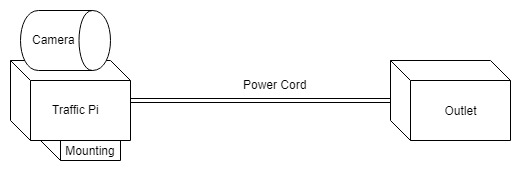
\includegraphics[width=0.90\textwidth]{images/Conceptual_Drawing.jpg}
    \caption{Traffic Pi conceptual drawing}
\end{figure}

\newpage
\section{Product Description}
\setlength{\parskip}{0.5em}
\noindent The primary function of the Traffic Pi is to use computer vision and object recognition to calculate the speed of a vehicle crossing the screen. We plan to mount an IR/Visible light camera along with a Raspberry Pi on the side of the road to allow regular citizens to perform their own traffic study. Our team has considered many risks such as environmental hazards and potential theft and plan to house our product inside a weather-proof, 3D-printed container.

\noindent With our product, we hope to find a solution to the massive costs of a standard traffic study—which includes hiring an engineer to lay cables to monitor the traffic on a street over a 24 hours period—with a computer vision-based product that will cost less and provide more information about vehicles passing through the designated study zone.

\noindent From a user's perspective, there will be very little setup required to begin conducting their own traffic study. Should the user need any help with configuration, our web page will provide adequate information to help walk the user through installing their Traffic Pi. Along with installation information, we will provide the user with an interface to manage any footage captured or data collected by the device. We will give the user the ability to see information such as how frequently vehicles passed through the area, how fast they were going, and even the actual vehicle that passed through the frame.

\noindent Alternatively, as a maintainer or administrator of the project, one should be able to provide a reliable service with the ability to self-update the Traffic Pi should the need for software management or troubleshooting arise. Our product will give administrators the ability to push any updates to the device software, force a restart of a device should a user need help with their device freezing or crashing, and general control by giving the user an interface to conduct low-level maintenance to the device. \par

\subsection{Features \& Functions}
\graphicspath{ {./images/} }
Traffic Pi main function is to detect and determine the speed of passing cars from a mantled raspberry pi (Figure 1) and document the information in a database. Detection will be processed through an IR/Visible light camera (Figure 2) that will be able to detect in both bright and dark environments. By user demand, the Traffic Pi will return documented data comprised of footage, speeds, time of day, and traffic activity. The data will be able to display through a user interface accessible on the customer’s personal computer including the ability to access the device through the cloud. Traffic Pi can also be able to connect to the internet to allow the ability to perform software updates. Traffic Pi’s main functionality is to detect and calculate the speed of passing cars, so the device will not function for the purpose of security nor will detect the activities outside of cars (i.e. pedestrians walking by). \newline\newline
Figure 1\newline
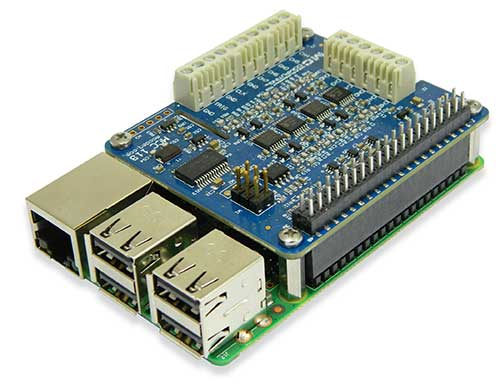
\includegraphics[width=14cm, height=10cm]{rasppi.jpg}\newline
Figure 2\newline
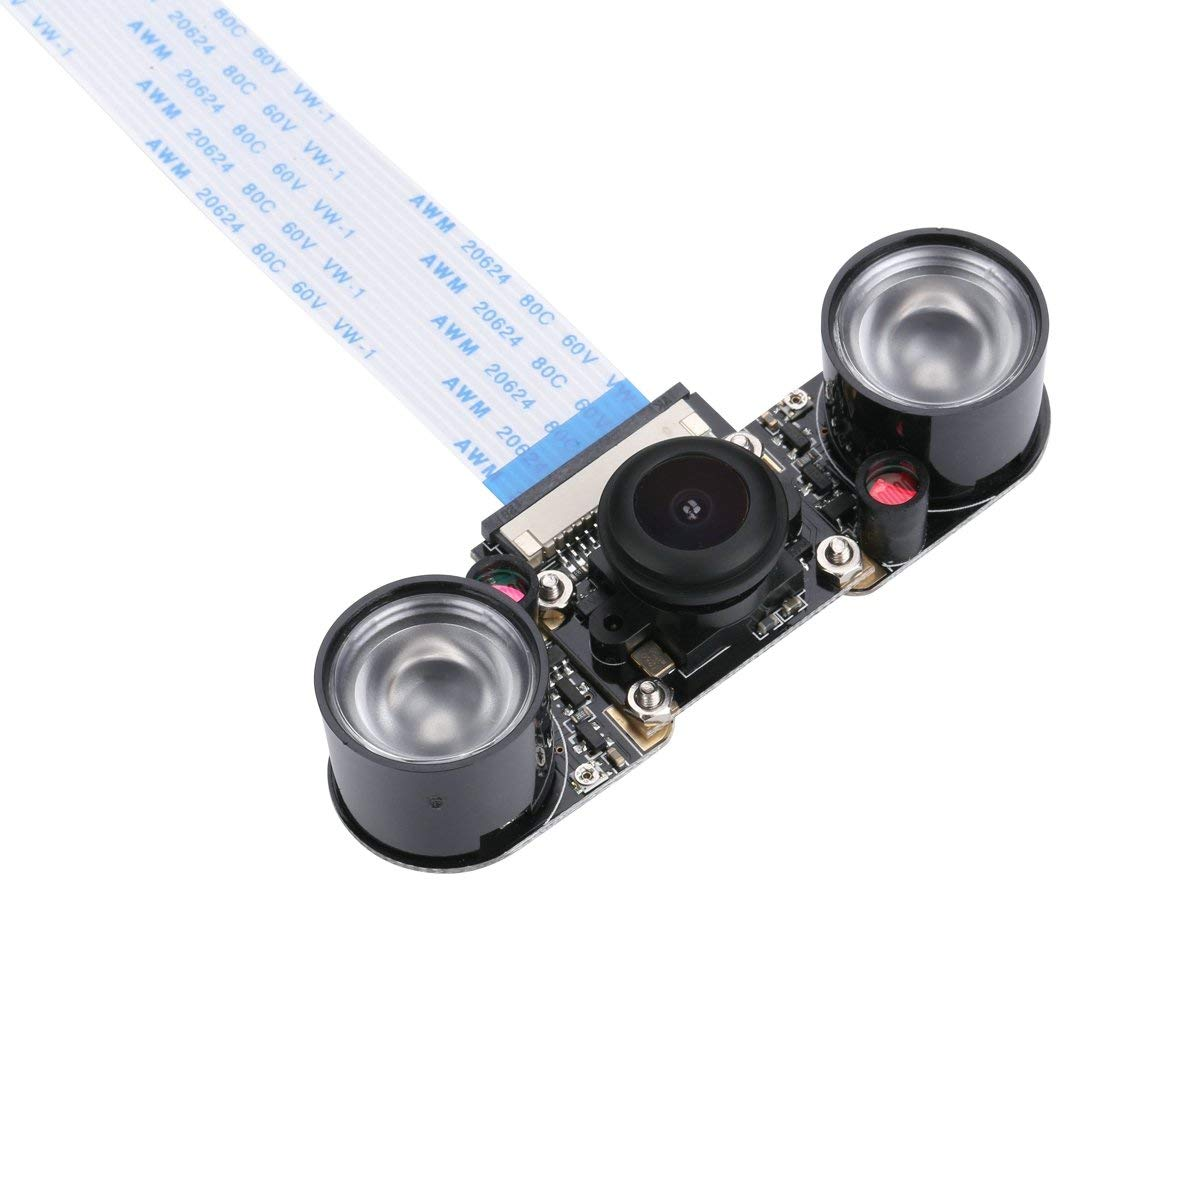
\includegraphics[width=14cm, height=10cm]{IR_camera.jpg}\newline

\subsection{External Inputs \& Outputs}
\begin{table}[h]
\centering
\resizebox{\textwidth}{!}{
\begin{tabular}{|l|l|l|}
\hline
 \textbf{Name} & \textbf{Description} & \textbf{Use}\\ \hline
 Arducam Noir  &  This will provide the video feed for the Traffic PI & Input \\ \hline
 Data Analytics & Captured data will be broken down and analyzed by a few metrics and uploaded to a cloud service & Output \\ \hline
 GUI & Data will be presented neatly to the user & Output \\ \hline
\end{tabular}}
\caption{Overview of External Inputs and Outputs}
\end{table}
\subsection{Product Interfaces}
\graphicspath{ {./images/} }
Homepage of the Traffic Pi website.\newline

\includegraphics[width=14cm, height=10cm]{1-Home.png}\newline
Main dashboard page for end user.\newline
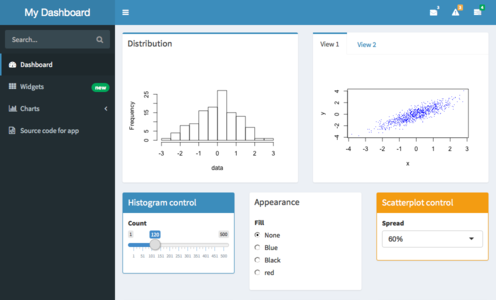
\includegraphics[width=14cm,height=10cm]{dashboard_1.png}\newline
Secondary dashboard page.\newline
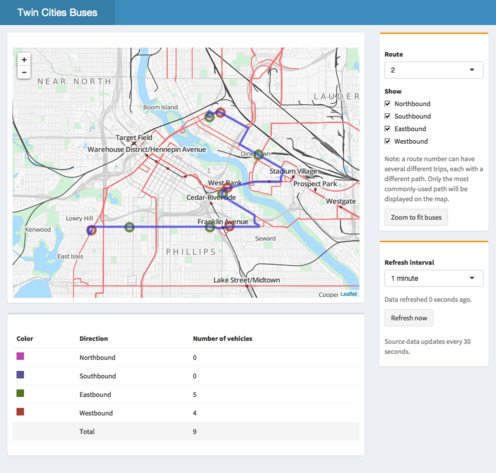
\includegraphics[width=14cm,height=10cm]{dashboard_2.png}\newline
\newpage
\section{Customer Requirements}
The customer requirements for Traffic Pi are those that were deemed to be the core essentials of this project by the team stakeholder, Dr. McMurrough. Each of the customer requirements described below define a function of the Traffic Pi system either in use, post-use, or as a commercial product. Each of the requirements defined below are critical to the Traffic Pi and can be used as a benchmark for determining the success of this system.

\subsection{Find Vehicle}
\subsubsection{Description}
The program should be able to find a vehicle inside of the frame. This means that if there are multiple cars in the frame at the same time, the second car's position and speed should not affect the position and speed of the first car. 
\subsubsection{Source}
Customer
\subsubsection{Constraints}
One assumption that may need to be made is that the entire car can fit into the frame. If it is too big (camera too close) it could negatively impact the calculation of our algorithm. 
\subsubsection{Standards}
We will use YOLOv3 as our image recognition software, so we will follow any standards they recommend using.
\subsubsection{Priority}
Critical

\subsection{Track Vehicle}
\subsubsection{Description}
The program should be able to track a vehicle inside of the frame. This means that if there are multiple cars in the frame at the same time, the second car's position and speed should not affect the position and speed of the first car. 
\subsubsection{Source}
Customer
\subsubsection{Constraints}
One assumption that may need to be made is that the entire car can fit into the frame. If it is too big (camera too close) it could negatively impact the calculation of our algorithm. 
\subsubsection{Standards}
We will use YOLOv3 as our image recognition software, so we will follow any standards they recommend using.
\subsubsection{Priority}
Critical

\subsection{Calculate Speed of Vehicle}
\subsubsection{Description}
The program will be able to calculate the speed the car is moving by determining the distance between two points and using a pixel to distance algorithm for each frame. 
\subsubsection{Source}
Customer
\subsubsection{Constraints}
Assume the ability to constantly detect the vehicle from when they enter the frame to when they exit the frame.
\subsubsection{Standards}
N/A
\subsubsection{Priority}
Critical

\subsection{Interface}
\subsubsection{Description}
Traffic Pi will provide a simple interface (web or otherwise) to display the data collected. 
\subsubsection{Source}
Customer
\subsubsection{Constraints}
N/A
\subsubsection{Standards}
N/A
\subsubsection{Priority}
Critical

\subsection{Cost}
\subsubsection{Description}
Traffic Pi will cost a reasonable amount to develop.
\subsubsection{Source}
Customer
\subsubsection{Constraints}
This strongly depends on the current cost of materials on the market
\subsubsection{Standards}
N/A
\subsubsection{Priority}
Moderate

\subsection{Affordability}
\subsubsection{Description}
Traffic Pi to be affordable to the average consumer
\subsubsection{Source}
Customer
\subsubsection{Constraints}
N/A
\subsubsection{Standards}
N/A
\subsubsection{Priority}
Moderate

\subsection{Mounting}
\subsubsection{Description}
The housing case for the Traffic Pi shall be designed such that it allows a user to connect a tripod or other mounted equipment to the Traffic Pi.
\subsubsection{Source}
Customer
\subsubsection{Constraints}
N/A
\subsubsection{Standards}
The mounting area has an area that fits to standard mounting plate designs
\subsubsection{Priority}
Critical

\subsection{Marketability}
\subsubsection{Description}
The Traffic Pi will be unique in its design and appealing to the public.
\subsubsection{Source}
Customer
\subsubsection{Constraints}
N/A
\subsubsection{Standards}
N/a
\subsubsection{Priority}
Critical

\subsection{Ease of use}
\subsubsection{Description}
Goal is to minimize the user interaction with the system
\subsubsection{Source}
Customer
\subsubsection{Constraints}
N/a
\subsubsection{Standards}
N/a
\subsubsection{Priority}
High
\newpage
\section{Packaging Requirements}
The Traffic Pi will come as a ready to deploy system. This means that upon delivery of the system to a customer, the only setup required by the customer is to turn on the system, point the device's camera at the area of interest (either through use of a tripod or using the Traffic Pi's mounting area to mount to a surface), and engage the system. The Traffic Pi will come preloaded with the software needed to run the system as well as interface with the offsite server.

\subsection{Information Website}
\subsubsection{Description}
Our project will include a webpage with information regarding information about setting up the device and maintaining the device. It will also include information regarding the scope of the project and what our reasoning is.
\subsubsection{Source}
Jacob Devasier
\subsubsection{Constraints}
N/A
\subsubsection{Standards}
N/A
\subsubsection{Priority}
Moderate

\subsection{Boxing}
\subsubsection{Description}
The Traffic Pi hardware will be packaged neatly before it's sold to the customer like any other commercial product
\subsubsection{Source}
Miguel Fraire
\subsubsection{Constraints}
N/A
\subsubsection{Standards}
N/A
\subsubsection{Priority}
Moderate
\newpage
\section{Performance Requirements}
Performance is vital to our program because we will need a high frames per second count to accurately calculate the speed of a vehicle passing by. To make this easier, we will use YOLO for the object recognition. YOLO is great for this because it only passes over the image once to look for a vehicle, so it has very little load on the device itself. This would allow us to reach a higher FPS than if we used other object recognition algorithms. Another important performance requirement is that we will have to record at least 24 hours of video for the study. To help this, one idea we have mentioned is caching the video is memory and only saving it when a vehicle is detected moving through the frame.

\subsection{Accurate speed calculation}
\subsubsection{Description}
We need to keep at least 30, but ideally 60 fps to make sure that our algorithm calculates the speed accurately.
\subsubsection{Source}
Jacob Devasier
\subsubsection{Constraints}
N/A
\subsubsection{Standards}
N/A
\subsubsection{Priority}
Moderate

\subsection{Power}
\subsubsection{Description}
Traffic Pi will provide a stable source of power using the standard 120 V
\subsubsection{Source}
Seth Tisbi
\subsubsection{Constraints}
N/A
\subsubsection{Standards}
N/A
\subsubsection{Priority}
Critical

\subsection{Database}
\subsubsection{Description}
Traffic Pi shall be able to store in a database the metadata collected from the 24 hour capture period
\subsubsection{Source}
Seth Tisbi
\subsubsection{Constraints}
The user's local computer may not have sufficient storage space to host the database.
\subsubsection{Standards}
N/A
\subsubsection{Priority}
Critical

\subsection{IR Camera}
\subsubsection{Description}
The IR camera used shall be able to operate as specified in little to no light scenarios.
\subsubsection{Source}
Seth Tisbi
\subsubsection{Constraints}
N/A
\subsubsection{Standards}
The IR camera has to be hold to its own specifications.
\subsubsection{Priority}
Critical

\subsection{3D Camera}
\subsubsection{Description}
The 3D camera used shall be able to operate as specified
\subsubsection{Source}
Seth Tisbi
\subsubsection{Constraints}
N/A
\subsubsection{Standards}
The 3D camera has to hold to its own specifications.
\subsubsection{Priority}
Critical

\subsection{Pi Storage}
\subsubsection{Description}
The Raspberry Pi shall have sufficient storage space to be able to store all video captured in a 24 hour period.
\subsubsection{Source}
Seth Tisbi
\subsubsection{Constraints}
At the end of a 24 hour period, the system depends on the user to offload the data stored on the Pi to a local computer and thus free space.
\subsubsection{Standards}
N/A
\subsubsection{Priority}
Critical

\subsection{Pre-processing}
\subsubsection{Description}
The application shall not commit to local memory video containing any cars.
\subsubsection{Source}
Seth Tisbi
\subsubsection{Constraints}
N/A
\subsubsection{Standards}
N/A
\subsubsection{Priority}
High

\subsection{Post-processing}
\subsubsection{Description}
The application will store all processed data on the users local machine
\subsubsection{Source}
Miguel Fraire
\subsubsection{Constraints}
N/A
\subsubsection{Standards}
N/A
\subsubsection{Priority}
High

\subsection{Local Storage}
\subsubsection{Description}
Traffic Pi shall commit to memory on the users computer the 24 hour video period.
\subsubsection{Source}
Seth Tisbi
\subsubsection{Constraints}
It is assumed and necessary that the user connect the Traffic Pi system to the local computer through a USB cable.
\subsubsection{Standards}
N/A
\subsubsection{Priority}
High
\newpage
\section{Safety Requirements}
To make sure our product is safe enough for public use, we will package our device in a 3D-printed shell with a transparent material for the camera to view from. We are still discussing what the transparent layer for the camera will be, but we will need to make sure that it will not shatter if the Traffic Pi is hit by a vehicle or dropped. Our product will likely use infrared lights to be able to view cars coming at night, but it will not be of any concern to users. 

\subsection{Usage}
\subsubsection{Description}
Traffic Pi will provide a basic manual displaying the correct and safe usage of the unit.
\subsubsection{Source}
Seth Tisbi
\subsubsection{Constraints}
N/A
\subsubsection{Standards}
N/A
\subsubsection{Priority}
Critical

\subsection{Cooling}
\subsubsection{Description}
Traffic Pi shall be able to stay within safe operating temperatures when in use.
\subsubsection{Source}
Seth Tisbi
\subsubsection{Constraints}
N/A
\subsubsection{Standards}
N/A
\subsubsection{Priority}
Critical

\subsection{Ventilation}
\subsubsection{Description}
The housing case for the Traffic Pi shall be designed such that it allows heat generated by the system to safely dissipate away from the system.
\subsubsection{Source}
Seth Tisbi
\subsubsection{Constraints}
N/A
\subsubsection{Standards}
N/A
\subsubsection{Priority}
High
\newpage
\section{Maintenance \& Support Requirements}
The main maintenance challenge for Traffic Pi will be servicing faulty equipment once it has been shipped to the customer. This does not mean that rigorous testing will not be performed however. Software patches pushed from the information website to a faulty Traffic Pi will be able to fix software related issues. Employees from the company will be able during normal business hours to answer questions from concerned customers concerning the product. The information website will have a section dedicated to common questions, potentially common fixes to faulty systems, and basic steps in maintaining the device. A demonstration video will also be provided to aide in the usage of the Traffic Pi by the customer.

\subsection{Information Website}
\subsubsection{Description}
Our project will include a web page with information regarding information about setting up the device and maintaining the device. It will also include information regarding the scope of the project and what our reasoning is
\subsubsection{Source}
Jacob Devasier
\subsubsection{Constraints}
We will only have support for English support, so we assume the user will be able to read and understand English.
\subsubsection{Standards}
N/A
\subsubsection{Priority}
Moderate

\subsection{Documentation Website}
\subsubsection{Description}
We will include a web page containing information regarding code documentation.
\subsubsection{Source}
Jacob Devasier
\subsubsection{Constraints}
Our choice will be slightly limited in scope based on our programming language of choice. Most documentation applications support C++ documentation and exporting to and HTML format, so we do not expect this to be a very heavy constraint.
\subsubsection{Standards}
TBD
\subsubsection{Priority}
Low

\subsection{Demonstration Video}
\subsubsection{Description}
Provided with our web page, we will record and present a demonstration video showing off some of the features of the Traffic Pi and how to use them.
\subsubsection{Source}
Jacob Devasier
\subsubsection{Constraints}
Once again the instructions and demonstration will be provided in English.
\subsubsection{Standards}
TBD
\subsubsection{Priority}
Low

\subsection{Interface Server}
\subsubsection{Description}
Traffic Pi will use a reliable server to host the website
\subsubsection{Source}
Seth Tisbi
\subsubsection{Constraints}
N/A
\subsubsection{Standards}
N/A
\subsubsection{Priority}
Low
\newpage
\section{Other Requirements}
A portion of the Traffic Pi physical assembly unit will have a section that will make mounting of the system to a physical environment easier. There are no other requirements for the Traffic Pi system. The core requirements are present in the Customer Requirements section as specified by the stakeholder, Dr. McMurrough. Other requirements that are encountered over the development of this system will be systematically added to this section.

\subsection{Pi Placement}
\subsubsection{Description}
The Pi shall have a set position to occupy while recording that faces the road.  It shall have a clip to attach itself to roofs or mailboxes in order to keep it steady, secure, and able to view enough of the road to collect accurate data.
\subsubsection{Source}
Ethan Duff
\subsubsection{Constraints}
The availability of use-able surfaces or ledges
\subsubsection{Standards}
N/A
\subsubsection{Priority}
High
\newpage
\section{Future Items}
The future of Traffic Pi is a cloud connected network of devices deployed across a city. Each deployed system would be able to network with a cloud server that in turn could network with other Traffic Pi systems across the city. Together the combined system's would be able to given a city-wide analysis of traffic. Further, the processing for such a system would occur on the cloud server.

\subsection{Compatibility With Cloud System}
\subsubsection{Description}
Optimally, a future version of the product should be able to record its data and then send the long video files to a system on the cloud.  This system will then run the programs that will actually analyze and record the traffic data from the Raspberry Pi.  This means that the Pi should be able to accurately and efficiently communicate without sources of different Operating Systems.
\subsubsection{Source}
Ethan Duff
\subsubsection{Constraints}
There are no relevant constraints for this requirement, though that is subject to change.
\subsubsection{Standards}
N/A
\subsubsection{Priority}
Low


\subsection{Pi Network}
\subsubsection{Description}
Should the product become a success a possible direction to take the project would be into networked Pi's.  Multiple Pi's would be set across the city and monitor many relevant intersections to gather a much wider and more diverse data set relevant to many different portions of a city at many different times.
\subsubsection{Source}
Ethan Duff
\subsubsection{Constraints}
Hardware constraints only.
\subsubsection{Standards}
Only the legal standards enforced by any given city.
\subsubsection{Priority}
Low
\newpage

%%% References
\bibliographystyle{plain}
\bibliographystyle{reference/IEEEtran_custom}
\bibliography{reference/refs}{}

\end{document}